\section{Software development} \label{sec:software-devel}
As we have explained previously, the slave device we are developing on this project needs some custom functionality that needs to be programmed.
The following sections will present and explain the algorithms and techniques used during development of each software module that compose the final control program.

The presentation of the several modules will mostly follow the order by which they were developed in order to better explain the programming logic and challenges we had to overcome during the process.

The way the software was designed and implemented from the start allows anyone to create different versions of each programmed module.
So long as the original API is retained, no additional modifications are needed on the modules that make such API function calls, meaning a direct swapping of modules can be performed.

The proposed and implemented software architecture can be seen in a block diagram format in \autoref{fig:sw-architecture}, shown previously on this chapter.

% Slave node software
% `- DFR0592 driver
\subsection{DFR0592 driver}
The first software module we started to develop was the 'driver` library that interacts with the DC motor control board, the DFRobot's DFR0592.
The communication with the DFR0592 is done via the I\textsuperscript{2}C channel and is based on registers.
If we want to read a value on register X, we simply send the register address we want to read and the board responds with the corresponding value.
If, instead, we wish to write a value, we also send the register address but with the most significant bit of the transmitted byte set to 1, which indicates a write operation (as opposed to a read operation, when it is 0), followed by the value we want to be written.

We began by testing the device functionality with a Python \cite{sw:python} script provided by the manufacturer.
We used it mostly to get a sense of what parameters and variables were needed to set the motor speed and get the speed feedback value, but also to get acquainted to how the I2C communication transactions worked.

It was at this stage that we found out the speed calculation algorithm implemented on the board was too slow to be used in a control loop because it only updated the feedback value once every 100ms.
This is what lead us to decide and change the encoder connection to the Raspberry Pi's GPIO pins and create our own encoder 'driver` and speed/position calculation algorithm.
This way we will have more flexibility on the feedback calculation algorithm, being able to run it with virtually any period.

After making sure our prototype communication algorithm was working correctly in Python, we began to 'translate` it to the C programming language.
Naturally some modification had to be made, especially because C is an event-oriented language, as opposed to Python which is mainly object-oriented.
We overcame this by creating a C struct with the same object data that we used in the Python prototype, paired with helper functions that perform the same operations as the Python's object methods.
The developed C functions all take, at least, one argument: a pointer to a variable of type \verb|struct dfr_board|, which is a pseudo-object representing a DFR0592 board.
\autoref{lst:dfr_struct} is an excerpt of the header file containing the definition of said struct.

\lstinputlisting[float=htp,language=C,firstline=24,lastline=31,caption=Definition of the DFR0592 pseudo-object C struct,label=lst:dfr_struct]{../src/DFR0592/dfr0592.h}

Each DFR0592 board comes pre-configured with the I\textsuperscript{2}C address \verb|0x10| but they can be changed, meaning several of these boards can be used simultaneously.
As such, the library was designed in a way that, in future works, one can communicate with several boards simultaneously.

The mentioned approach was used in order to mimic the working principle of an object-oriented programming language in C.
This was mostly useful on the libraries that may need to manage several pseudo-objects of the same type (e.g. the PID algorithm library), but we used the same principle throughout all code-base, for consistency reasons.

% `- GPIO encoder 'driver'
\subsection{Raspberry Pi's GPIO encoder driver}
After having determined the best approach for speed and position measurement was to connect the motor encoder to the GPIO of the Raspberry Pi, it prompted us to develop a dedicated driver to handle the input signals.
The designed driver converts the logical values from the quadrature encoder signals A and B into a step sequence by mapping the A/B pair of values onto a sequence number, as shown in \autoref{table:encoder-ab-sequence}.

\begin{table}[htp]
	\centering
	\caption{Encoder step sequence mapping}
	\label{table:encoder-ab-sequence}
	\begin{tabular}{|c|c|c|}
		\hline
		A & B & sequence  \\
		\hline
		0 & 0 & 0         \\
		\hline
		1 & 0 & 1         \\
		\hline
		1 & 1 & 2         \\
		\hline
		0 & 1 & 3         \\
		\hline
	\end{tabular}
\end{table}

To gain software access to the GPIO lines on the Raspberry Pi, the Linux C library \verb|libgpiod| \cite{lib:libgpiod} was used.
This library allows two modes of acquiring input values: periodic polling and event-triggered action.
Our implementation uses periodic polling, in which the new update of values will be triggered by the main control task, following its cyclic period.
The event-triggered action will call a specified function whenever the configured input(s) line changes its value, either from boolean 0 to 1 or 1 to 0.

The periodic polling approach was easy to prototype and implement but it will have less precision when working with slow speeds, meaning an implementation based on event-triggered actions could be implemented as future work, in order to improve both performance and measurement precision in slow speeds.
As we were mostly interested in creating a proof-of-concept system, we accepted the reduced precision on slower speeds, in exchange for the simplest and smallest implementation.

After the encoder signals are mapped to the sequence number, a counter variable is updated after every polling iteration, according to the difference between the current and previous sequence numbers.
If the sequence number increases, the counter is incremented by the same amount, and vice versa.
When the sequence number wraps around in either direction the counter value is only changed by 1, meaning when it jumps from 3 to 0, the counter is incremented by 1, and is decremented when the sequence number jumps from 0 to 3.
This counter value will later be used in the speed and position computation library.
Every iteration its value will be compared with the previous and, combined with the necessary ratios (the encoder's Pulses per Revolution (PPR) and the motor gearbox ratio), the motor's instantaneous speed and position are estimated for the current time-step.

Again, for consistency reasons, this software library was designed to mimic the object-oriented programming style and thus it's possible to use multiple encoders simultaneously.

% `- speed/position calculation algorithm
\subsection{Speed and position algorithm}
Even though this algorithm was implemented as a separate library from the encoder driver, it heavily relies on data from said driver.
Having it implemented as a separate module means a different algorithm can be developed and be used as a swap-in replacement for the current one.

The current implementation works as a stand-alone cyclic task that performs the following actions (see \autoref{fig:pv-module-steps} for a graphical representation):
\begin{enumerate}
	\item fetches the above mentioned encoder counter variable from the encoder module;
	\item fetches the current internal clock timestamp and calculates the time delta from the last iteration; \label{misc:pvstep2}
	\item calls the internal \verb|_calc_position()| function, that applies the configured encoder scale, gearbox ratio and transforms the value into degrees;
	\item calls the internal \verb|_calc_velocity()| function, that applies the same scales but also uses the time delta calculated in step \ref{misc:pvstep2} to convert the value to speed, in Revolutions per Minute (RPM);
	\item saves the current timestamp as the previous one, to be used on the next iteration;
\end{enumerate}

\begin{figure}[htp]
	\centering
	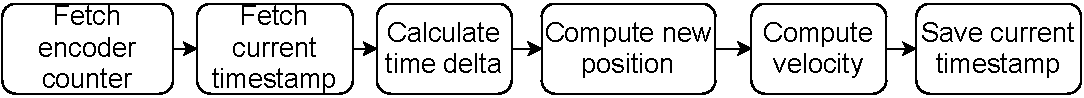
\includegraphics[width=0.8\linewidth]{pv_module_steps.pdf}
	\caption{Overview of the module cyclic steps}
	\label{fig:pv-module-steps}
\end{figure}

Following the same design pattern of the previous modules, a C struct variable is used to store the pseudo-object data, including the calculated speed and position values.
A such, a more complex system that may need to calculate speeds and positions for multiple motors simultaneously can be implemented with this library, due to the mimicking of an object-oriented implementation.

Even though the data struct is transparent to outside of the library, public functions are provided to fetch these values.
These functions include an interlock variable to control the access to the memory regions where such values are stored (the \verb|pthread mutex| implementation is used), to make sure the cyclic calculation task is not disrupted by any external fetch operations.
This is a common technique used in multi-threaded software where concurrent running parts of the same software application need to access the same memory location, but naturally they cannot do it simultaneously.

% `- PID algorithm
\subsection{PID control algorithm}
In order to perform any type of movement control, either it being speed, position, or any other, some form of control algorithm needs to be used.
To this effect, we are going to use the most common control algorithm in the control universe: the Proportional/Integral/Derivative (PID) controller.
Virtually everyone in the controls universe is familiar with the PID controller and its working principle:

\begin{itemize}
	\item It receives two inputs: a reference value and a feedback value;
	\item Computes the error between the two, meaning how far is the current value (the feedback) from the desired value (the reference);
	\item The Proportional term will contribute to the output value according to the calculated error;
	\item The Integral term will contribute to the output value according to the accumulated error over time;
	\item The Derivative term will contribute to the output according to the error's rate of change.
\end{itemize}

Because we did not want to spend to much time implementing something that already has a lot of different implementations, we have programmed a simple library with a PID algorithm based on the one used in the LinuxCNC \cite{sw:linuxcnc} project.
It has not been ported into our project, instead we implemented our own version of the same algorithm and design, with the exception that we applied the design pattern of using a C structure for holding the pseudo-object data.
In this case, multiple PID controllers can be implemented simultaneously using the same library.
This was an important characteristic to have as position control requires controllers for both the position and speed, simultaneously.

During the testing phase the implementation demonstrated a good performance and correctness.
As such, we accepted its usage for our proof-of-concept prototype, but admit a better algorithm or implementation might be necessary for a production release.

% `- netHAT handler
\subsection{netHAT 52-RTE handler library}
The Hilscher's netHAT 52-RTE board already includes support for the C programming language, provided by a library.
As such, we did not have the need to develop a driver in the general sense of controlling the board behaviour.
Instead we have created a `handler' library that makes the proper calls to the driver's functions and stores the cyclically updated data onto a C struct, the same concept of storing the pseudo-object data as before.
Even though the netHAT boards are not designed to allow multiple simultaneous connections, we still used this approach for consistency reasons.

Limiting the code-base that directly interacts with external drivers or APIs is a common technique to ease the development process and to allow faster and better error tracing.
Having the netHAT driver functions confined to a restrict set of helper functions allows us to maintain a clean coding style.
In the event of bugs or even API changes to the library, all driver calls are centralised in a single place, allowing one to correct bugs and make modifications or improvements that influence the entire software, without having to navigate all code-base looking for references to the driver's API.

The \verb|comm| library we have implemented takes care of all interactions with the netHAT 52-RTE driver and maintains a local copy of the cyclically synchronised data, the previously referred 32 bytes of inputs and 32 bytes of outputs.
Functions are provided to automatically perform the following actions:

\begin{enumerate}
	\item Initialise the SPI communication with the board and setup board and communication parameters; \label{misc:comm_step_1}
	\item Wait for the communication to be established (blocking function call) or, alternatively, check if the connection is active or not (non-blocking function call); \label{misc:comm_step_2}
	\item Synchronise the input data with the network (update the local copy with the network data);
	\item Fetch input data, either a single bit, a byte or a word (two bytes), from the local copy;
	\item Set output data, either a single bit, a byte or a word (two bytes), on the local copy;
	\item Synchronise the output data with the network (send the modified local data copy to the network); \label{misc:comm_step_6}
	\item Stop the SPI communication and `shutdown' the board. \label{misc:comm_step_7}
\end{enumerate}

\begin{figure}[htp]
	\centering
	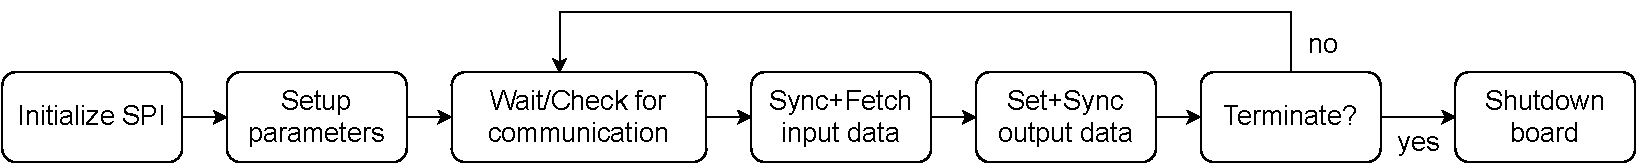
\includegraphics[width=0.8\linewidth]{comm_module_steps.pdf}
	\caption{Overview of the `comm' module cyclic steps}
	\label{fig:comm-module-steps}
\end{figure}

The actual behaviour of the slave device will naturally be determined by the main control loop but this library was to designed to start the execution on step \ref{misc:comm_step_1}, then loop steps \ref{misc:comm_step_2} through \ref{misc:comm_step_6} during normal execution, and terminate with step \ref{misc:comm_step_7}, as shown graphically in \autoref{fig:comm-module-steps}.

% `- main control loop
\subsection{Main control task}
Following the already implemented design pattern, the main control task will also use a C struct to store its pseudo-object variables.
The current implementation is only prepared to run a single instance, although running multiple could be achieved, if that is something that makes sense for a particular experiment.
Nonetheless, care must be taken creating multiple instances as no verification mechanisms have been implemented for simplicity reasons.

This task will not implement any new features to the control application itself.
Instead, its purpose is to maintain a periodic loop and trigger the actions that need to be performed at each time-step iteration, meaning this is where the top-level logic of the slave device is implemented.
All actions are achieved via function calls to the libraries presented earlier and all information that needs to be transferred between modules is done via this control task.

As this control application is being developed in the year 2021, where even inexpensive computing platforms include multi-core processors (such as the Raspberry Pi), its has been designed from the start with multi-threading in mind.
Multi-threading is a simpler approach to simultaneous processing by giving the same process (application) multiple execution threads that may perform computations simultaneously.
Compared to multi-processing, where several different processes (applications) work together to achieve some goal, data sharing is much simpler because threads within the same process share the same memory address-space (the system memory allocated exclusively for the process) \cite{technology:mp-vs-mt}.
While allowing all threads to access all available data within the process is faster than having to transmit said data to other processes, explicit synchronisation of memory access is required to ensure that multiple threads do not try to access the same memory region simultaneously, which will very likely corrupt such data.
This has been implemented via the usage of mutual exclusion (mutex) pseudo-objects.
In particular, we used the mutex implementation from the Linux \verb|pthreads| library, which we also used to create and manage the several execution threads of the control application.

The final top-level logic implemented in this module is the following:

\begin{enumerate}
	\item Lock the \verb|comm| module configuration (via the \lstinline[columns=fixed]|comm_bus_config_lock()| function); \label{misc:main-logic-step-lock-config}
	\item Acquire the current timestamp; \label{misc:main-logic-step-acquire-timestamp}
	\item Order the \verb|comm| module to update the inputs via the \lstinline[columns=fixed]|comm_update_inputs()| function;
	\item Check if the EtherCAT communication is active, if not then jump to step \ref{misc:main-logic-step-store-timestamp}; \label{misc:main-logic-step-check-active-comm}
	\item Read the \verb|enable| bit from the inputs, if it is false then jump to step \ref{misc:main-logic-step-store-timestamp}; \label{misc:main-logic-step-check-enabled}
	\item Copy the reference and feedback values to the PID pseudo-object;
	\item Perform the PID computations;
	\item Set the motor speed to the value of the PID output;
	\item Set the first two output words of the \verb|comm| module to the values of the feedback speed and position, respectively; \label{misc:main-logic-step-update-outputs}
	\item Store the current timestamp as the previous one, so that in the next iteration the `previous timestamp' already has the correct value; \label{misc:main-logic-step-store-timestamp}
	\item Order the \verb|comm| module to update the outputs;
	\item Sleep until the period time has been elapsed; \label{misc:main-logic-step-sleep}
\end{enumerate}

\begin{figure}[htp]
	\centering
	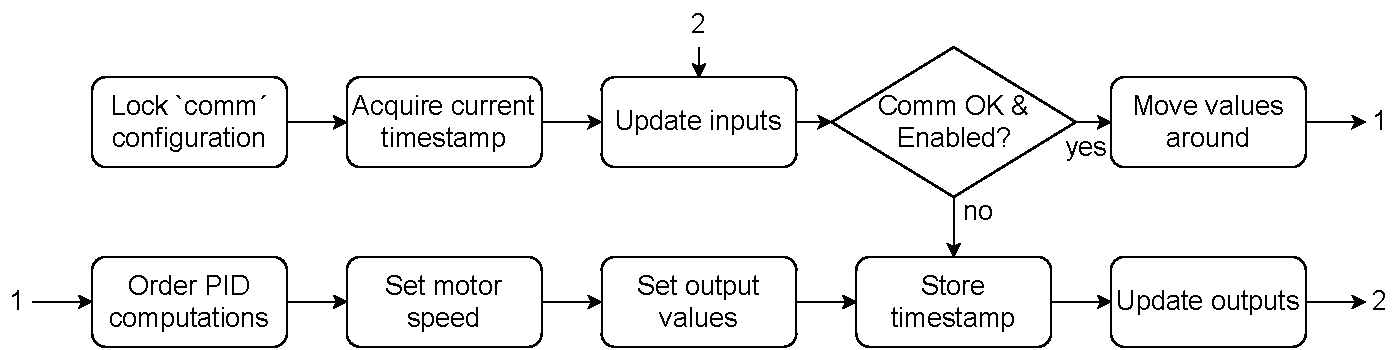
\includegraphics[width=0.8\linewidth]{control-module-steps.pdf}
	\caption{Overview of the control steps}
	\label{fig:control-module-steps}
\end{figure}

This logic is implemented so that the code starts at step \ref{misc:main-logic-step-lock-config} and then loops steps \ref{misc:main-logic-step-acquire-timestamp} through \ref{misc:main-logic-step-sleep}, taking into account the conditions on steps \ref{misc:main-logic-step-check-active-comm} and \ref{misc:main-logic-step-check-enabled}.
This logic can also be visualised in \autoref{fig:control-module-steps}.
The PID computations are only performed if running in local control mode, otherwise the motor speed is fetched from the RTE network, through the \verb|comm| module. 

% `- miscelaneous initialisation code
\subsection{Initialisation code and debug output}
At last but not least, before the main control task begins executing, all data structures and libraries need to be initialised.
For simplicity of implementation, dynamic parameters will be passed through a fixed format command-line argument list when launching the control application.
A list and a format representation of the parameters to be passed can be visualised by launching the \verb|main| executable without any arguments.

Contrary to what was initially planned, a module that would take care of exporting the performance data relating to the control application was not implemented.
Instead, in order to also minimise the amount of concurrent threads within the application, the exporting of debug data was implemented within the \verb|pid| module.
During development we realised that during each time-step all relevant data for exportation was already stored on the PID pseudo-object, so it made sense to include the exporting functions on the same module.
The main module was planned to have the responsibility of initialising data and auxiliary threads and then terminating them, during the shutdown procedure, but during normal execution, no processing would be done in this thread.
As such, we ended up taking advantage of this unused thread and let the exporting of the debug data be performed on it.

The data exportation itself is a simple algorithm, called periodically from the \verb|main| thread, that appends the current PID pseudo-object data to a file with the Comma-Separated Values (CSV) format.
This file format is very simple and is based on the concept that different values on the same line are separated by commas and that they maintain the same relative horizontal position across all lines of the entire file \cite{sw:csv}.

\begin{small}
	\lstinputlisting[float=htp,basicstyle=\footnotesize,firstline=4,lastline=14,breaklines=true,
	caption=Excerpt from an experimental data CSV output file,label=lst:csv_data]{../data/local-5ms.csv}
\end{small}

